第3章で運転電圧を超えると、LGAD検出器の時間分解能が悪化する様子が見られた。
LGADの時間分解能は、タイムウォーク$\sigma_{\rm{tw}}$、ジッター$\sigma_{\rm{j}}$、ランダウノイズ$\sigma_{\rm{L}}$の3つが大きく影響すると考えられており、
式\ref{eq_TimingResolution} で示すことができる。
ジッターを構成する要素のノイズ $\sigma_{\rm{n}}$、立ち上がり時間$t_{\rm{r}}$、信号の大きさ$S$を測定して、式\ref{eq_Jitter_2} からジッターを計算して求めることができる。
ジッターが時間分解能の悪化に影響しているという推測の元、レーザー測定で求めた時間分解能と、計算から求めたジッターを比較することで、時間分解能を悪化する原因を調べる。
本章ではまず、ジッターを構成するノイズ、立ち上がり時間、信号の大きさを測定した。
その結果から、ジッターと時間分解能の増幅率依存性を評価し、増幅率が大きい時の時間分解能の悪化の原因について考察していく。

%そのため、ジッター$\sigma_j$のみによってLGAD検出器の時間分解能$\sigma_t$を評価することができる。

\section{立ち上がり時間の測定}
\subsection{解析方法}
図\ref{fg:RiseTime_analysis}にオシロスコープの信号の出力を示す。
横軸が時間、縦軸が波高で、黄色線がセンサーからの信号である。
最大波高の60%と40%の時の波高と時間の差を取ることで、最大波高の60%から40%の立ち上がり時間と波高差のデータを取得した。

%式 \ref{eq_Jitter} より、信号の傾き$\left|\frac{S}{t_r}\right|$はこのように求めることができる。
%そのため、立ち上がり時間$t_r$を波高の60%から40%の範囲の値を使用するので、信号の大きさ$S$も60%から40%の範囲の波高の差を用いる必要がある。

全イベントの取得したデータをヒストグラムにして、その時の最頻値を最大波高の60%から40%の立ち上がり時間$t_r$と波高差$S$とした。
PINの信号雑音比が小さいため、立ち上がり時間と波高差を求める際の範囲を広げすぎると、
ノイズの影響で立ち上がり時間と波高差を正しく解析することができないので、範囲を波高の60%から40%に設定した。


\begin{figure}[h]
    \centering
    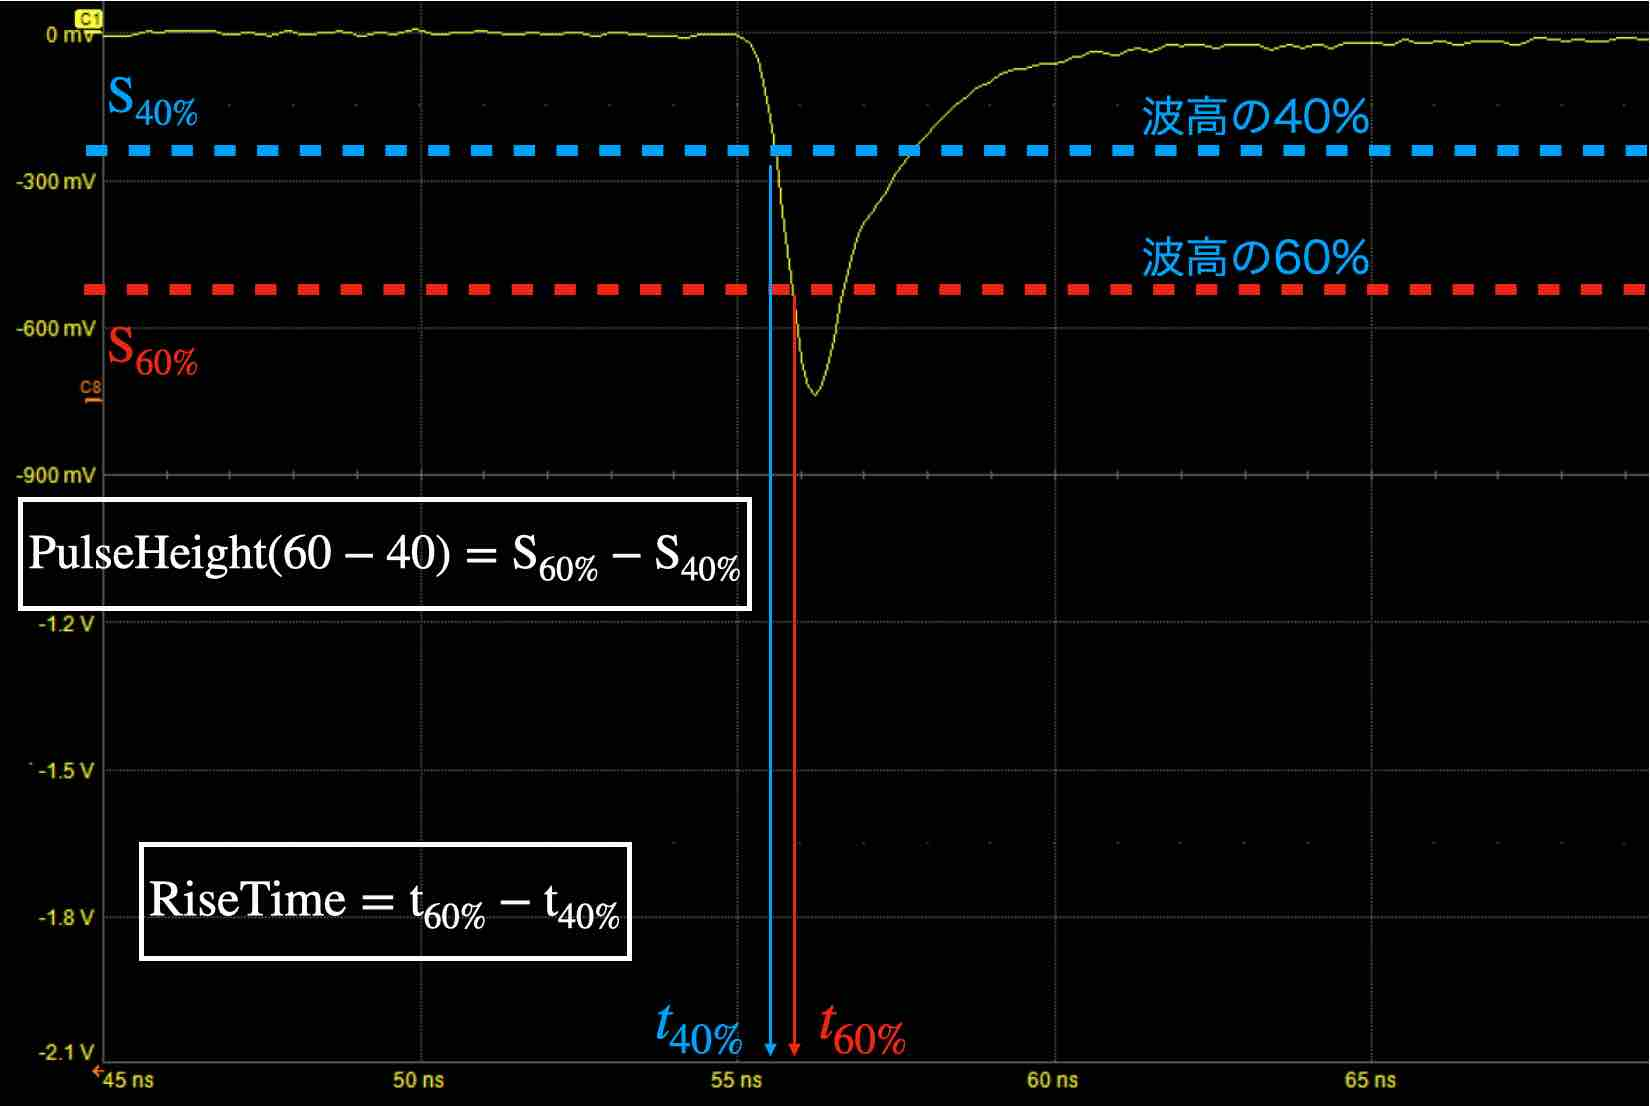
\includegraphics[width=10cm]{fig/ch4/RiseTime_analysis.jpg}
    \caption[立ち上がり時間の解析方法]{立ち上がり時間の解析方法\\横軸が時間、縦軸が波高で、LGADの信号が黄色線。\\最大波高の60%と40%の波高と時間の差をとって、立ち上がり時間$t_r$と60%から40%の波高の差$S$を求めた。}
    \label{fg:RiseTime_analysis}
\end{figure}

\begin{figure}[h]
    \begin{minipage}[b]{0.5\linewidth}
        \centering
        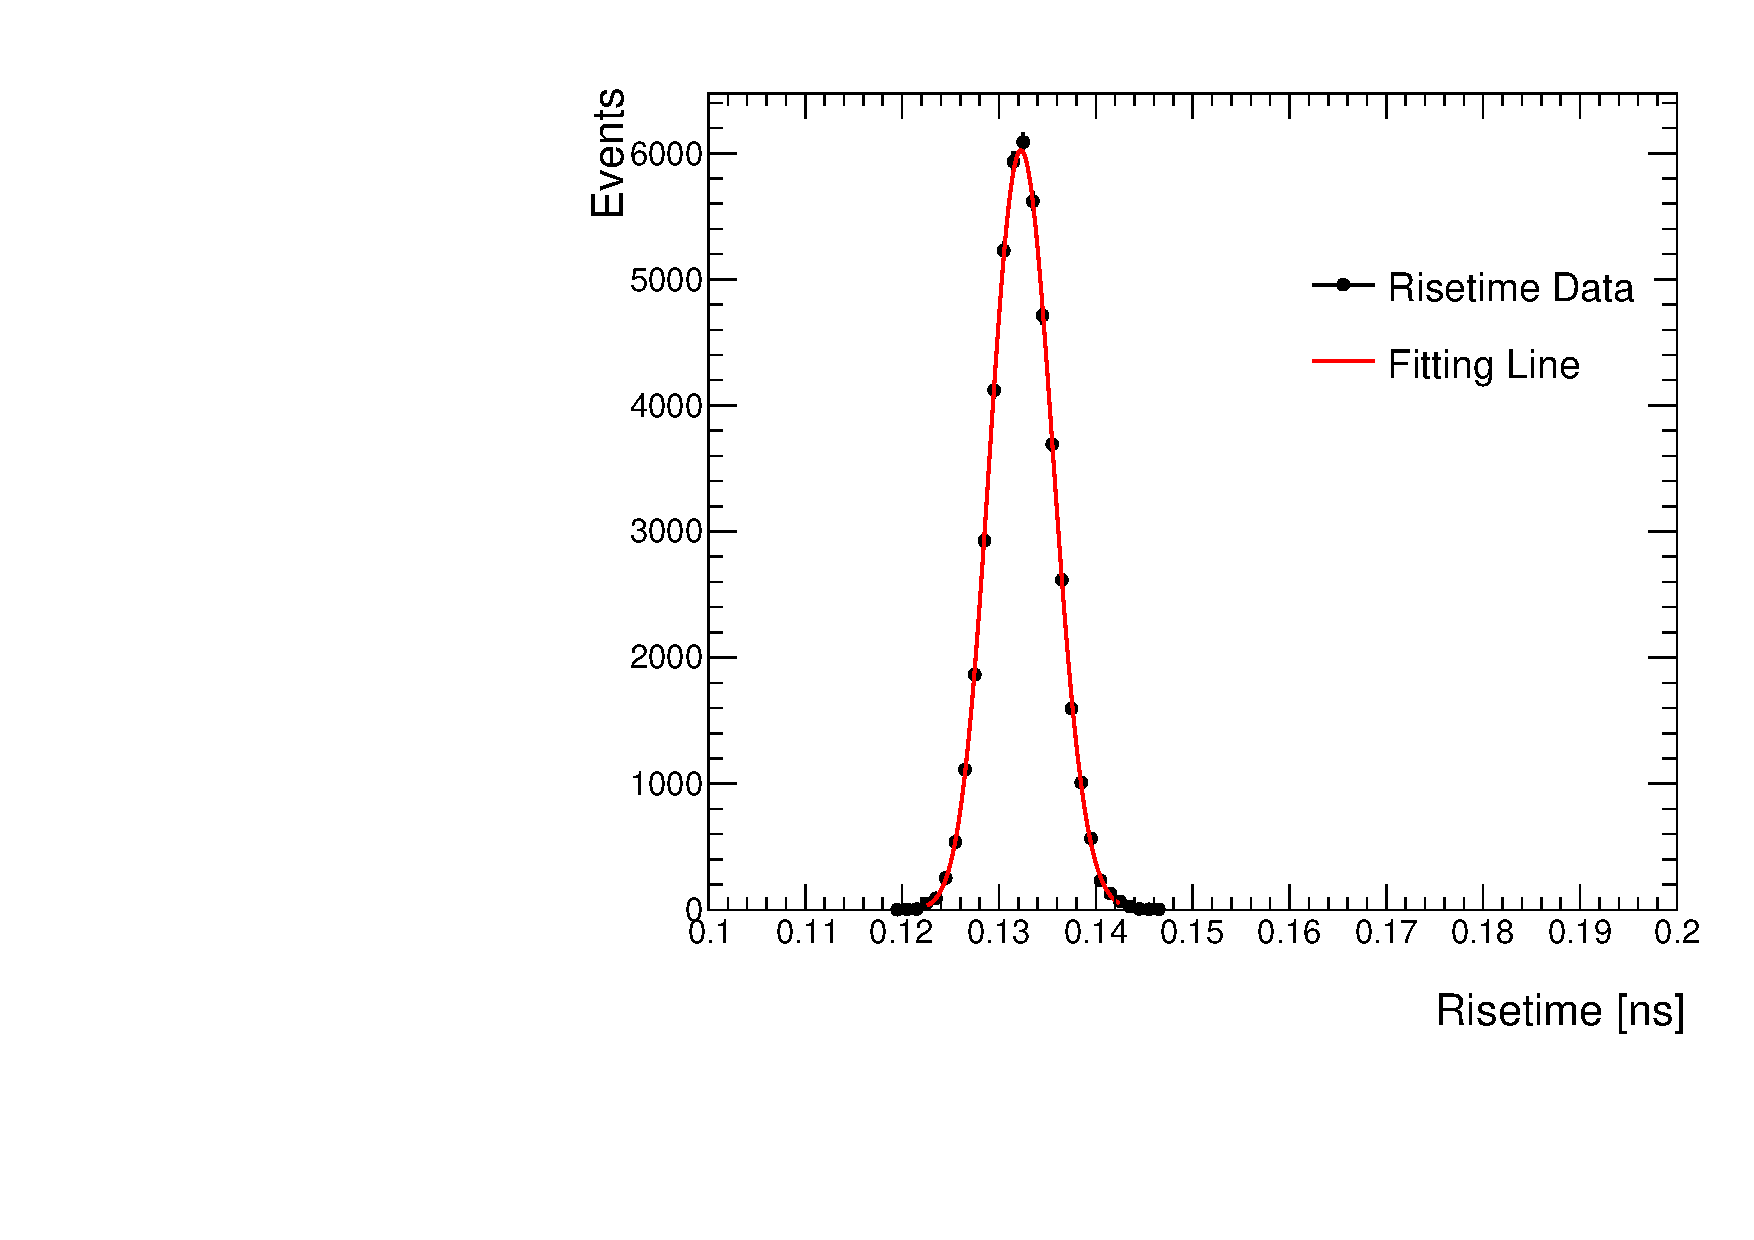
\includegraphics[width=8cm]{fig/graph/Risetime_hist_APD.pdf}
        \caption[立ち上がり時間のヒストグラム]{立ち上がり時間のヒストグラム\\最頻値を立ち上がり時間とした。}
        \label{fg:Risetime_hist_APD}
    \end{minipage}
    \begin{minipage}[b]{0.5\linewidth}
        \centering
        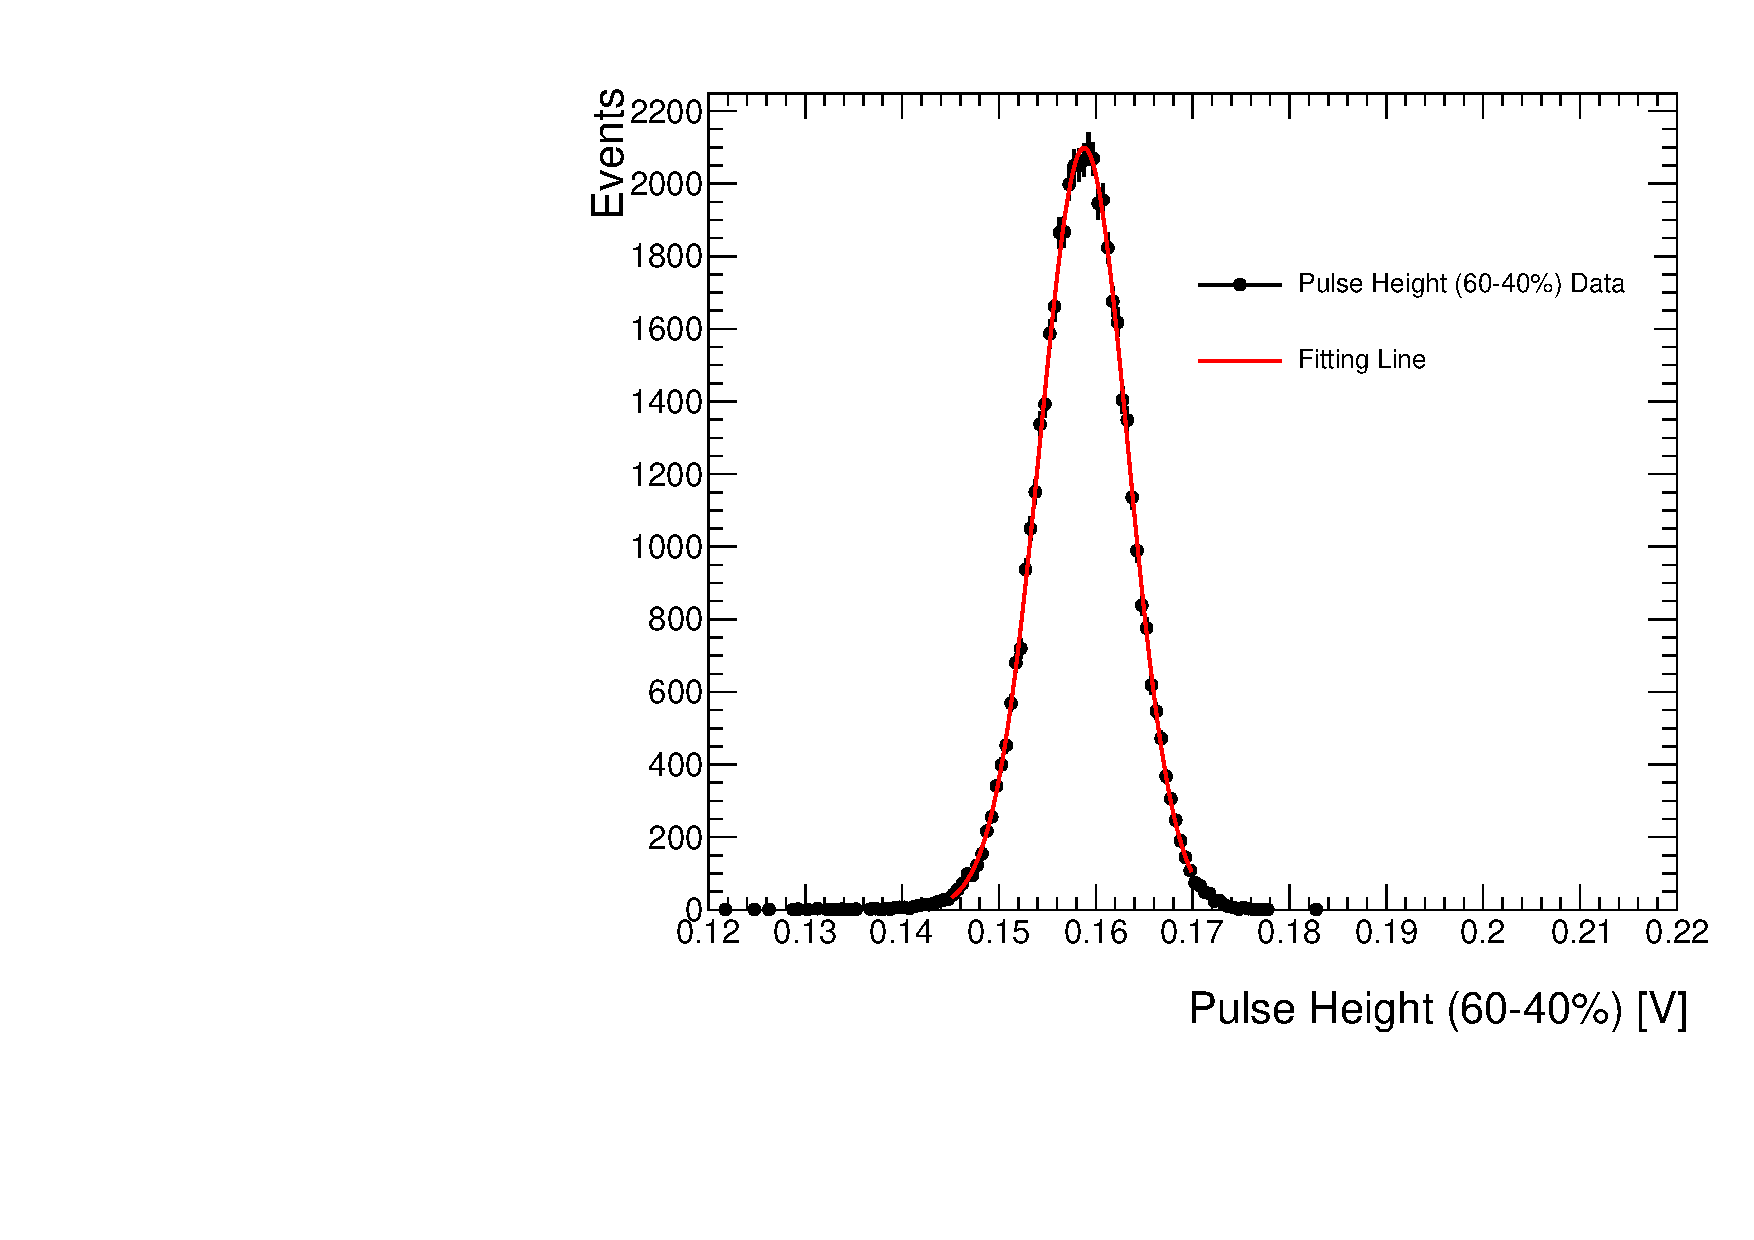
\includegraphics[width=8cm]{fig/graph/PulseHeight_hist_60-40.pdf}
        \caption[波高差のヒストグラム]{波高差のヒストグラム\\最頻値を波高の60%から40%の波高差とした。}
        \label{fg:APD_Ph_60-40_vsBias}
    \end{minipage}
\end{figure}

\begin{figure}[h]
    \centering
    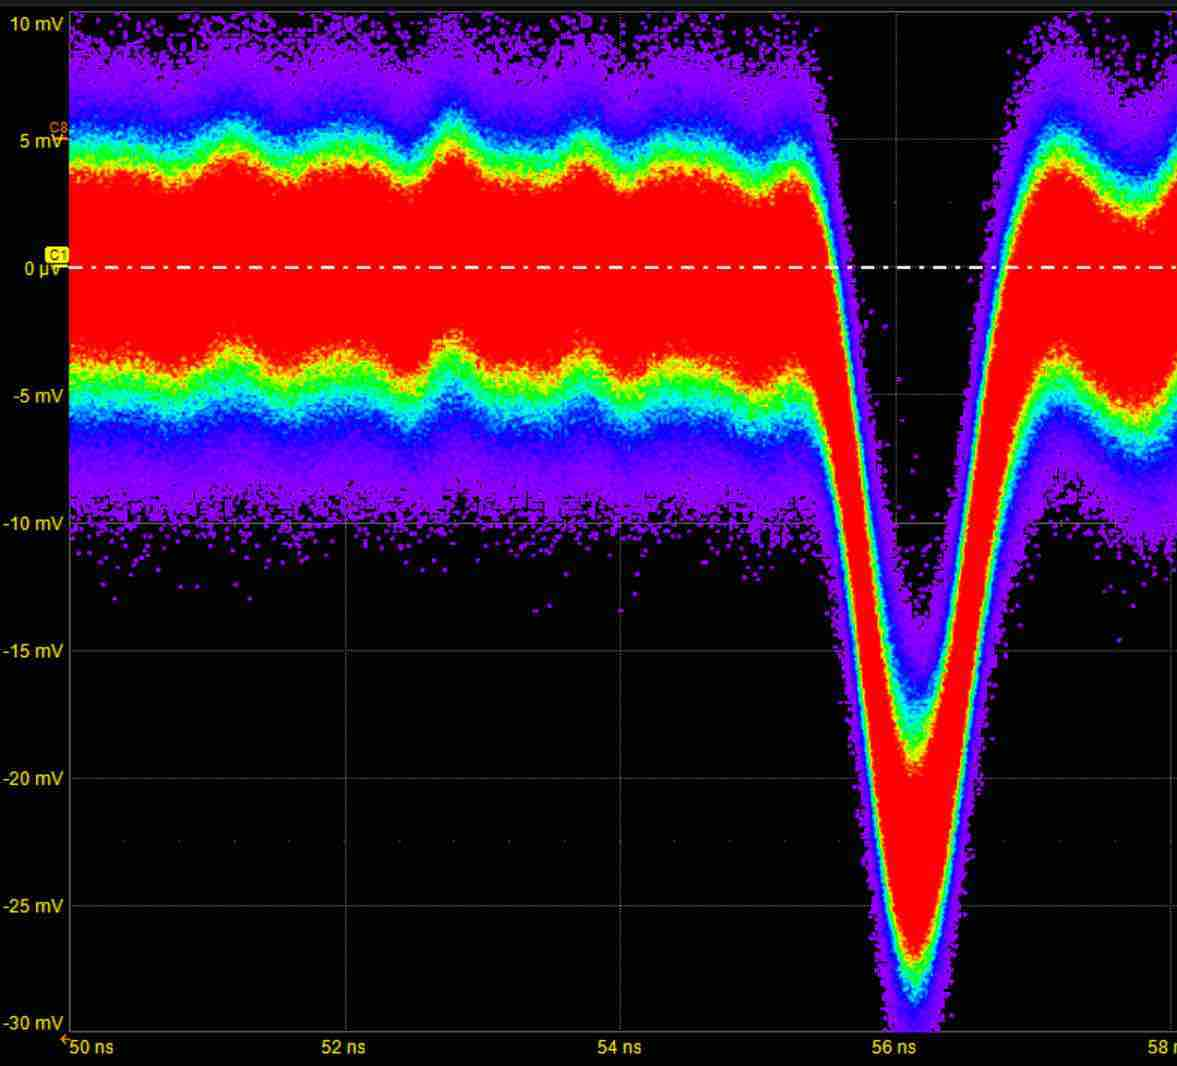
\includegraphics[width=6cm]{fig/ch5/PIN_波形_12.6.jpg}
    \caption[PINの波形]{PINの波形\\PINは信号雑音比が小さいため、ノイズの影響で立ち上がり時間と波高差を正しく解析することができないので、範囲を波高の60%から40%に設定した。}
    \label{fg:RiseTime_analysis}
\end{figure}

\subsection{立ち上がり時間の測定結果}
LGADとPINの立ち上がり時間の電圧依存性を 図\ref{fg:RiseTimevsBias} に示す。
横軸が電圧で、縦軸が立ち上がり時間で、赤点がLGADで、青点がPINの測定点である。
PINの立ち上がり時間の電圧依存性はほとんど一定であることがわかった。
これは、PINの波形が電圧を上げてもほとんど変わらないため、信号の立ち上がりの変化が小さいからであると考える。
LGADの立ち上がり時間は、電圧が大きくなると小さくなり、運転電圧を超えると悪化することがわかった。
運転電圧に近づくほど、LGADの信号の立ち上がりは速くなることがわかる。
運転電圧を超えると、立ち上がり時間が速くならない理由は、電子が飽和ドリフト速度に達するため、
これ以上、電子正孔対の速度が大きくならないことに加えて、ノイズが大きくなることによって、立ち上がり時間が悪化するのではないかと考える。

\begin{figure}[h]
    \centering
    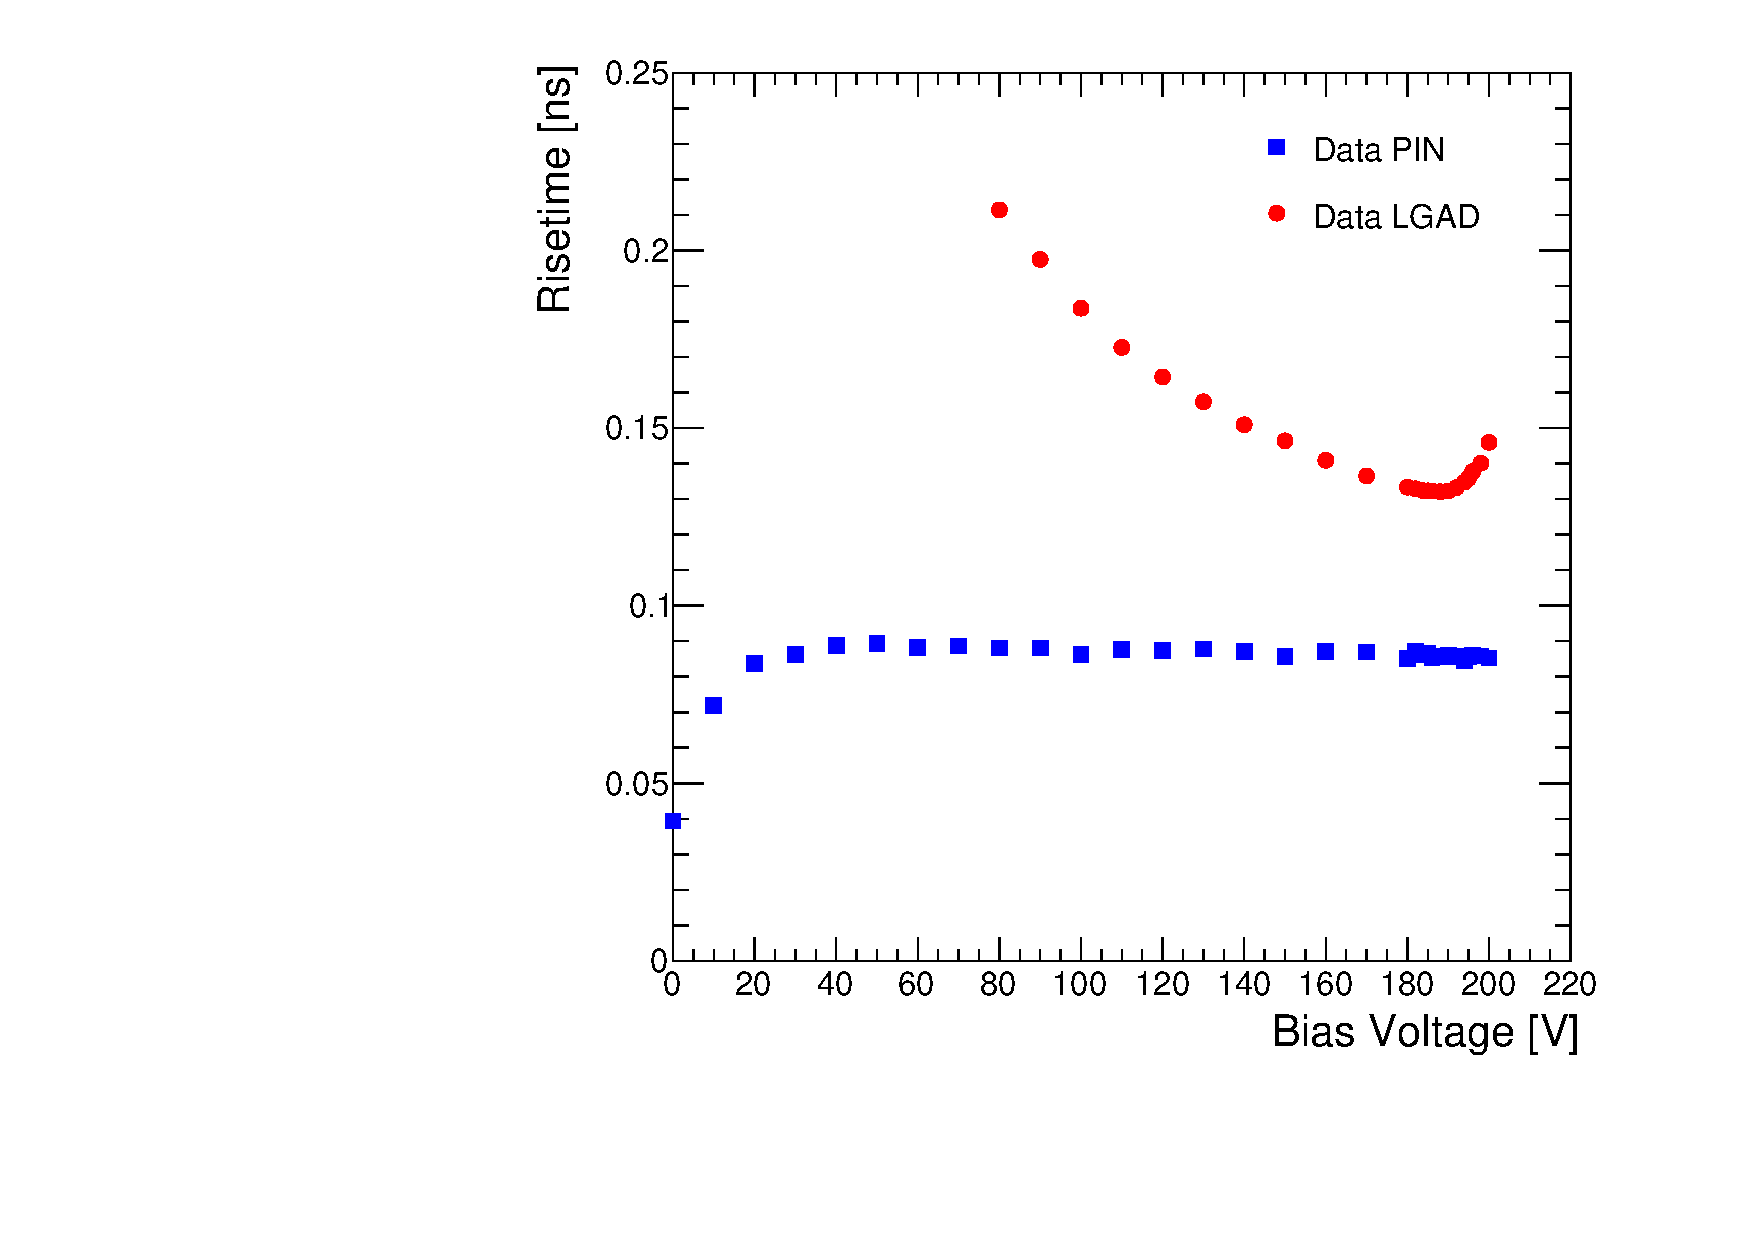
\includegraphics[width=10cm]{fig/graph/RisetimevsVoltage.pdf}
    \caption[AC-LGAD検出器の立ち上がり時間の電圧依存性]{AC-LGAD検出器の立ち上がり時間の電圧依存性\\横軸が電圧で縦軸が立ち上がり時間、赤点がLGADで青点がPINの測定点}
    \label{fg:RiseTimevsBias}
\end{figure}

\subsection{波高差の測定結果}
LGADとPINの波高差の測定から、x軸が印加電圧、y軸が波高差のグラフを作成した。
図\ref{fg:PIN_Ph_60-40_vsBias} はPINの波高差の電圧依存性で、図\ref{fg:APD_Ph_60-40_vsBias} はLGADの波高差の電圧依存性である。
PINのグラフは、図\ref{fg:PIN_MPVvsBias} の信号の大きさの電圧依存性のグラフと同様に、空乏化によって、波高差が変化する様子が見られた。
LGADのグラフは、図\ref{fg:APD_MPVvsBias} の信号の大きさの電圧依存性のグラフと同様に、増幅層による電子正孔対の増幅による、波高差の増加が見られた。

\begin{figure}[h]
    \begin{minipage}[b]{0.5\linewidth}
        \centering
        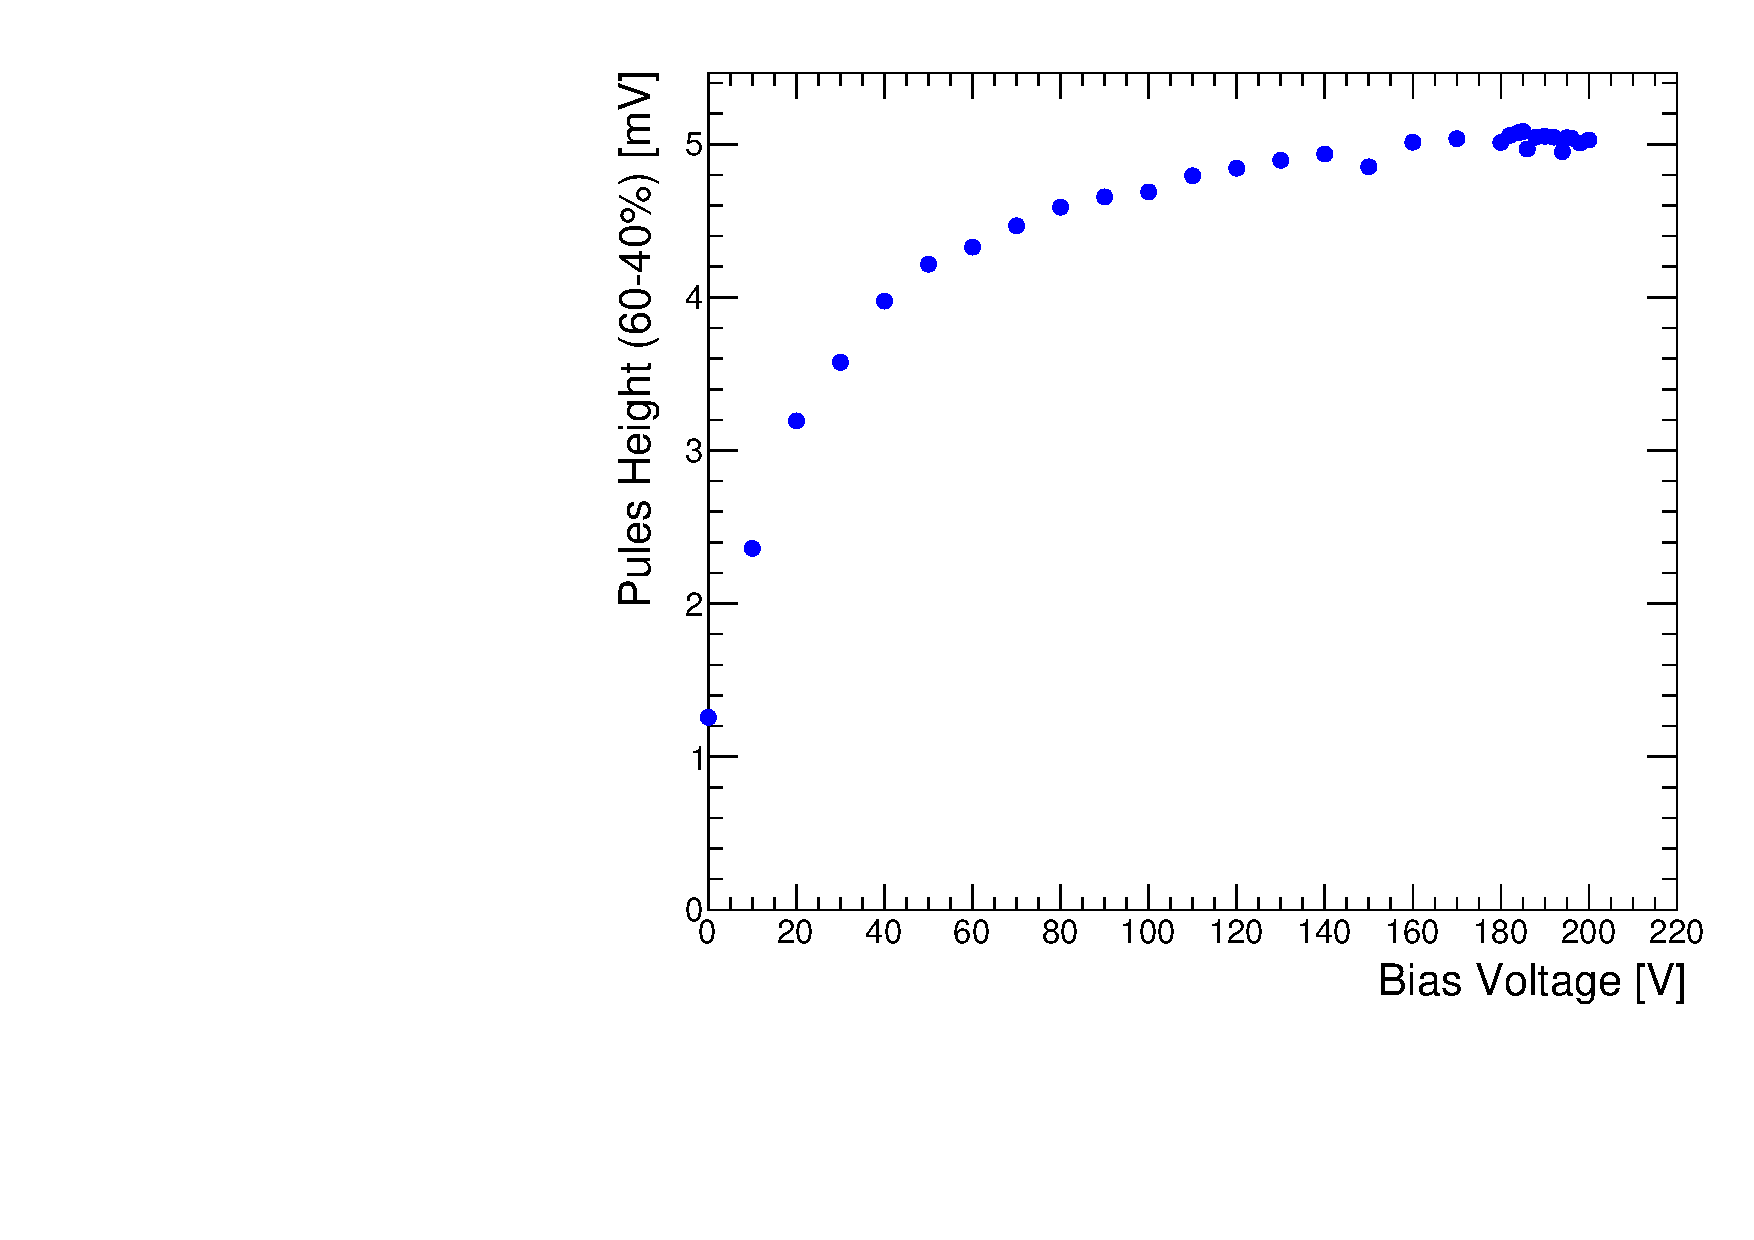
\includegraphics[width=8cm]{fig/graph/SignalSizevsVoltage_PIN_60-40.pdf}
        \subcaption{増幅層が無いPIN}
        \label{fg:PIN_Ph_60-40_vsBias}
    \end{minipage}
    \begin{minipage}[b]{0.5\linewidth}
        \centering
        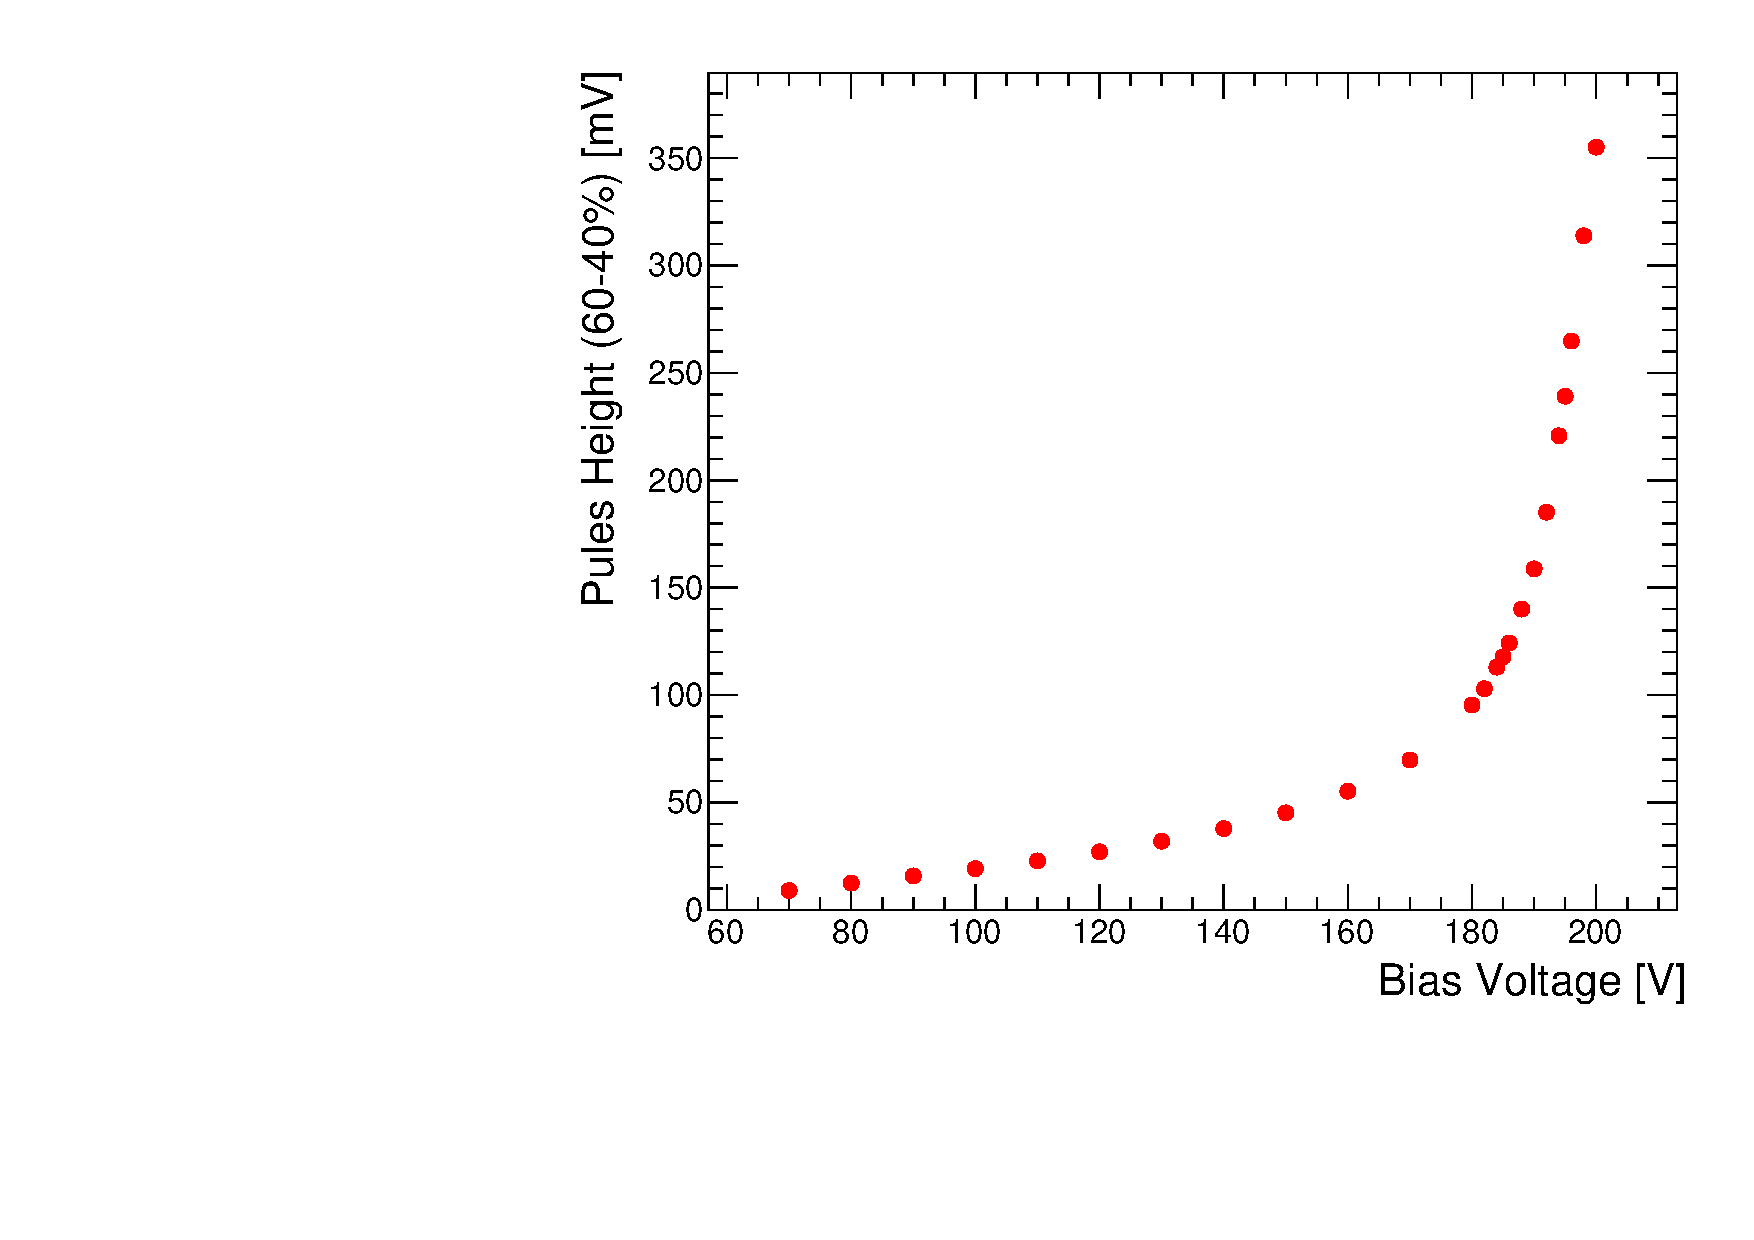
\includegraphics[width=8cm]{fig/graph/SignalSizevsVoltage_APD_60-40.pdf}
        \subcaption{増幅層が有るLGAD}
        \label{fg:APD_Ph_60-40_vsBias}
    \end{minipage}
    \caption[AC-LGAD検出器の波高の60%から40%の差の電圧依存性]{AC-LGAD検出器の波高の60%から40%の差の電圧依存性\\x軸が電圧でy軸が波高の60%から40%の差、赤点がLGAD検出器で、青点がPINの測定点}
\end{figure}
